\chapter{Normalization Layers}
La normalizzazione è una tecnica cruciale nell’addestramento di reti neurali profonde. Essa viene introdotta per migliorare l’ottimizzazione e stabilizzare l'apprendimento. In particolare, si fa riferimento alla \textbf{Batch Normalization (BN)} come metodo per affrontare problemi legati al cosiddetto \textit{internal covariate shift}.

\section{Covariate Shift}
Il \textbf{Covariate Shift} rappresenta un cambiamento nella distribuzione degli input tra il training e il test. Nelle CNN \textit{(Convolutional Neural Network)} (che vedremo nel capitolo successivo), i cambiamenti nei pesi degli strati inferiori modificano la distribuzione degli input per gli strati successivi, rallentandone pertanto l'addestramento. Questo fenomeno è noto come \textit{internal covariate shift}, un problema legato al fatto che ci si deve continuamente adattare a nuove distribuzioni, questa cosa inevitabilmente farà rallentare la convergenza.

\subsection{Problemi di Ottimizzazione}
La BN permette di normalizzare gli input degli strati intermedi, imitando un \textit{whitening} (decorrelazione con media zero e varianza unitaria). Questo processo è simile alla normalizzazione iniziale degli input delle reti, ma applicato a ogni batch durante l’addestramento.

\subsection{Perché il metodo classico non funziona}
Un approccio classico, allenare una rete e successivamente effettuare la normalizzazione, porta a fallire. Questo accade perché la normalizzazione effettuata post hoc, rompe il flusso del gradiente portando a bias esplosivi. La disconnessione fra ottimizzazione e normalizzazione causa dei problemi, per esempio il gradiente non tiene contro dell'effetto della normalizzazione. Pertanto una soluzione proposta è quella di inserire un layer di normalizzazione (Figura~\ref{fig:bn-layer}) all'interno del modello, in questo modo il gradiente lo "vede" e può essere in grado di correggere i parametri della rete in maniera coerente.
\begin{figure}
    \centering
    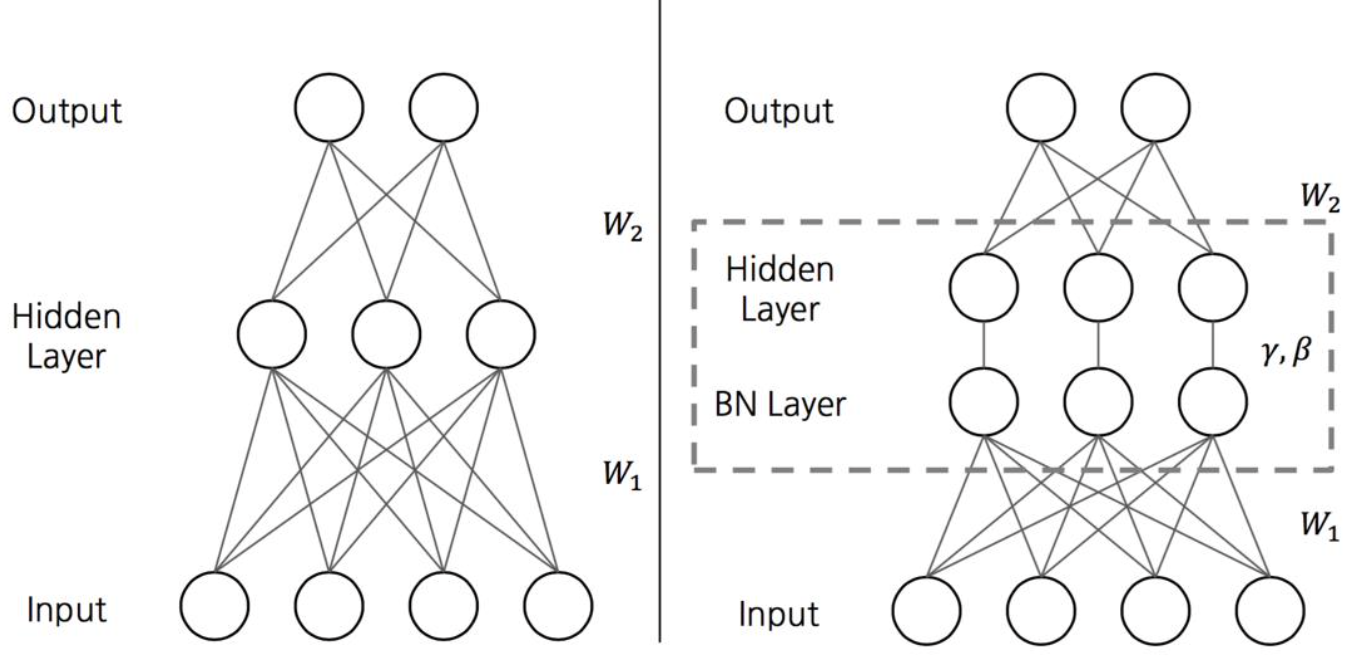
\includegraphics[width=0.85\linewidth]{figure/BNlayer.png}
    \caption{Inserimento di un layer utilizzando la Batch Normalization}
    \label{fig:bn-layer}
\end{figure}
\begin{quote}
“Il layer BN può imparare anche l’identità, rendendo reversibile la normalizzazione se necessario.”
\end{quote}

Analiziamo passo passo, quali sono i passaggi effettuati per giungere a ciò che ottimizza al meglio la Normalizzazione:
\begin{itemize}
  \item Ogni feature è normalizzata separatamente;
  \item Si usa la normalizzazione Z-score;
  \item Le stime di media e varianza vengono calcolate sul batch;
  \item Sono presenti due parametri appresi: $\gamma$ (scaling) e $\beta$ (bias), per mantenere la capacità rappresentativa.
\end{itemize}

Sia $x$ un input e $x^{(k)}$ la $k$-esima feature:

\begin{equation*}
    \mu^{(k)} = \frac{1}{m} \sum_{i=1}^m x_i^{(k)} \quad\quad \sigma^{2(k)} = \frac{1}{m} \sum_{i=1}^m (x_i^{(k)} - \mu^{(k)})^2
\end{equation*}
\begin{equation*}
    \hat{x}_i^{(k)} = \frac{x_i^{(k)} - \mu^{(k)}}{\sqrt{\sigma^{2(k)} + \epsilon}} \quad\quad y_i^{(k)} = \gamma^{(k)} \hat{x}_i^{(k)} + \beta^{(k)}
\end{equation*}

Se non ci fossero i due parametri $\beta$ e $\gamma$ la distribuzione dei valori di output, avrebbe una media nulla e una varianza unitaria e questa applicazione non sarebbe utile, pertanto questi due valori mantengono la forza rappresentativa della rete neurale complessiva.


\subsubsection{Perché la Batch Normalization è efficace}
\begin{itemize}
  \item Rende più stabili le distribuzioni di attivazione;
  \item Riduce l’effetto di gradienti esplosivi/vanescenti;
  \item Permette l’uso di learning rate più alti;
  \item Consente di usare attivazioni sature (e.g. sigmoid);
  \item Diminuisce la necessità di tecniche di regularizzazione;
  \item Riduce il tempo di training;
  \item Migliora la generalizzazione;
  \item Aumenta l'accuratezza.
\end{itemize}

Esistono inoltre varie tipologie di normalizzazione ed essi differiscono semplicemente per la dimensione del gruppo di campioni usati per la normalizzazione, per esempio lungo i canali, i batch presi in considerazioni o ancora la scelta di un singolo esempio.


\subsection{Conclusioni}

Sebbene la normalizzazione si sia dimostrata estremamente efficace nella pratica~\parencite{IoffeSzegedy2015BatchNorm}, le ragioni profonde del suo successo rimangono oggetto di dibattito nella comunità scientifica. L’ipotesi originale del \textit{covariate shift} interno, è stata messa in discussione da analisi successive~\parencite{Santurkar2018BNTheory}, che hanno mostrato come l’efficacia della normalizzazione derivi piuttosto dal miglioramento della geometria della funzione di costo e dalla maggiore stabilità durante l’ottimizzazione. In particolare:

\begin{itemize}
    \item Le reti che incorporano strati di normalizzazione risultano più semplici da ottimizzare, permettendo l’uso di tassi di apprendimento più elevati~\parencite{Santurkar2018BNTheory};
    \item La normalizzazione introduce una forma di rumore stocastico dovuto alla variabilità delle statistiche di batch, che agisce come un meccanismo implicito di regolarizzazione~\parencite{Bjorck2018UnderstandingBN};
    \item La procedura riduce la sensibilità all’inizializzazione dei pesi e stabilizza il processo di addestramento~\parencite{Bjorck2021BNStability};
    \item Infine, ha ispirato numerose varianti che estendono tali benefici a contesti differenti~\parencite{Ba2016LayerNorm, Wu2018GroupNorm}.
\end{itemize}

Nel complesso, la normalizzazione ha reso le architetture neurali più robuste, permettendo di combinare liberamente diversi blocchi e di addestrare reti profonde anche in condizioni di forte malcondizionamento numerico.
